% Options for packages loaded elsewhere
\PassOptionsToPackage{unicode}{hyperref}
\PassOptionsToPackage{hyphens}{url}
\PassOptionsToPackage{dvipsnames,svgnames,x11names}{xcolor}
%
\documentclass[
  ignorenonframetext,
]{beamer}
\usepackage{pgfpages}
\setbeamertemplate{caption}[numbered]
\setbeamertemplate{caption label separator}{: }
\setbeamercolor{caption name}{fg=normal text.fg}
\beamertemplatenavigationsymbolsempty
% Prevent slide breaks in the middle of a paragraph
\widowpenalties 1 10000
\raggedbottom
\setbeamertemplate{part page}{
  \centering
  \begin{beamercolorbox}[sep=16pt,center]{part title}
    \usebeamerfont{part title}\insertpart\par
  \end{beamercolorbox}
}
\setbeamertemplate{section page}{
  \centering
  \begin{beamercolorbox}[sep=12pt,center]{part title}
    \usebeamerfont{section title}\insertsection\par
  \end{beamercolorbox}
}
\setbeamertemplate{subsection page}{
  \centering
  \begin{beamercolorbox}[sep=8pt,center]{part title}
    \usebeamerfont{subsection title}\insertsubsection\par
  \end{beamercolorbox}
}
\AtBeginPart{
  \frame{\partpage}
}
\AtBeginSection{
  \ifbibliography
  \else
    \frame{\sectionpage}
  \fi
}
\AtBeginSubsection{
  \frame{\subsectionpage}
}
\usepackage{amsmath,amssymb}
\usepackage{lmodern}
\usepackage{iftex}
\ifPDFTeX
  \usepackage[T1]{fontenc}
  \usepackage[utf8]{inputenc}
  \usepackage{textcomp} % provide euro and other symbols
\else % if luatex or xetex
  \usepackage{unicode-math}
  \defaultfontfeatures{Scale=MatchLowercase}
  \defaultfontfeatures[\rmfamily]{Ligatures=TeX,Scale=1}
\fi
% Use upquote if available, for straight quotes in verbatim environments
\IfFileExists{upquote.sty}{\usepackage{upquote}}{}
\IfFileExists{microtype.sty}{% use microtype if available
  \usepackage[]{microtype}
  \UseMicrotypeSet[protrusion]{basicmath} % disable protrusion for tt fonts
}{}
\makeatletter
\@ifundefined{KOMAClassName}{% if non-KOMA class
  \IfFileExists{parskip.sty}{%
    \usepackage{parskip}
  }{% else
    \setlength{\parindent}{0pt}
    \setlength{\parskip}{6pt plus 2pt minus 1pt}}
}{% if KOMA class
  \KOMAoptions{parskip=half}}
\makeatother
\usepackage{xcolor}
\newif\ifbibliography
\usepackage{graphicx}
\makeatletter
\def\maxwidth{\ifdim\Gin@nat@width>\linewidth\linewidth\else\Gin@nat@width\fi}
\def\maxheight{\ifdim\Gin@nat@height>\textheight\textheight\else\Gin@nat@height\fi}
\makeatother
% Scale images if necessary, so that they will not overflow the page
% margins by default, and it is still possible to overwrite the defaults
% using explicit options in \includegraphics[width, height, ...]{}
\setkeys{Gin}{width=\maxwidth,height=\maxheight,keepaspectratio}
% Set default figure placement to htbp
\makeatletter
\def\fps@figure{htbp}
\makeatother
\setlength{\emergencystretch}{3em} % prevent overfull lines
\providecommand{\tightlist}{%
  \setlength{\itemsep}{0pt}\setlength{\parskip}{0pt}}
\setcounter{secnumdepth}{-\maxdimen} % remove section numbering
\usepackage{graphicx}
\usepackage{bm}
\usepackage{array}
\usepackage{amsmath}
\usepackage{amsthm}
\usepackage{amsfonts}
\usepackage{amssymb}
\usepackage{tikz-cd}
\usepackage{url}
\definecolor{foreground}{RGB}{255,255,255}
\definecolor{background}{RGB}{34,28,54}
\definecolor{title}{RGB}{105,165,255}
\definecolor{gray}{RGB}{175,175,175}
\definecolor{lightgray}{RGB}{225,225,225}
\definecolor{subtitle}{RGB}{232,234,255}
\definecolor{hilight}{RGB}{112,224,255}
\definecolor{vhilight}{RGB}{255,111,207}
\setbeamertemplate{footline}[page number]
\ifLuaTeX
  \usepackage{selnolig}  % disable illegal ligatures
\fi
\IfFileExists{bookmark.sty}{\usepackage{bookmark}}{\usepackage{hyperref}}
\IfFileExists{xurl.sty}{\usepackage{xurl}}{} % add URL line breaks if available
\urlstyle{same} % disable monospaced font for URLs
\hypersetup{
  pdftitle={STAT 528 - Advanced Regression Analysis II},
  pdfauthor={Exponential family theory (part 4)},
  colorlinks=true,
  linkcolor={Maroon},
  filecolor={Maroon},
  citecolor={Blue},
  urlcolor={blue},
  pdfcreator={LaTeX via pandoc}}

\title{STAT 528 - Advanced Regression Analysis II}
\author{Exponential family theory (part 4)}
\date{}
\institute{Daniel J. Eck\\
Department of Statistics\\
University of Illinois}

\begin{document}
\frame{\titlepage}

\begin{frame}
\newcommand{\R}{\mathbb{R}}
\newcommand{\Prob}{\mathbb{P}}
\newcommand{\Proj}{\textbf{P}}
\newcommand{\Hcal}{\mathcal{H}}
\newcommand{\rootn}{\sqrt{n}}
\newcommand{\p}{\mathbf{p}}
\newcommand{\E}{\text{E}}
\newcommand{\Var}{\text{Var}}
\newcommand{\Cov}{\text{Cov}}

\newtheorem{cor}{Corollary}
\newtheorem{lem}{Lemma}
\newtheorem{thm}{Theorem}
\newtheorem{defn}{Definition}
\newtheorem{prop}{Proposition}
\end{frame}

\begin{frame}{Last time}
\protect\hypertarget{last-time}{}
\begin{itemize}
\tightlist
\item
  generalized linear models (GLMs)
\item
  different parameterizations
\item
  motivation of logistic regression
\item
  inference for model parameters
\item
  comparing models
\end{itemize}
\end{frame}

\begin{frame}{Learning Objectives Today}
\protect\hypertarget{learning-objectives-today}{}
\begin{itemize}
\tightlist
\item
  Optimization
\item
  Sufficiency
\item
  Maximum Entropy
\item
  Wrap-up
\end{itemize}
\end{frame}

\begin{frame}{Background}
\protect\hypertarget{background}{}
We start with a regular full exponential family with log likelihood \[
  \langle y,\theta \rangle - c(\theta)
\] where \(\theta,y \in \mathbb{R}^n\). We have a canonical linear
submodel where

\begin{itemize}
\tightlist
\item
  \(\theta = M\beta\)
\item
  \(\beta \in \mathbb{R}^p\)
\item
  \(p < n\)
\end{itemize}

and log likelihood \[
  \langle M'y, \beta \rangle - c_\beta(\beta).
\]
\end{frame}

\begin{frame}{}
\protect\hypertarget{section}{}
A depiction of the transformations necessary to change between
parameterizations.

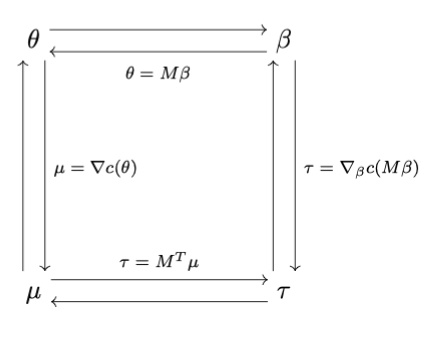
\includegraphics{transformations.png}
\end{frame}

\begin{frame}{}
\protect\hypertarget{section-1}{}
The only way to determine the MLEs is to maximize the log likelihood \[
  \langle M'y, \beta \rangle - c_\beta(\beta).
\] to obtain \(\hat\beta\) and then

\begin{itemize}
\tightlist
\item
  \(\hat\theta = M\hat\beta\)
\item
  \(\hat\mu = \nabla c(\hat\theta)\)
\item
  \(\hat\tau = M^T\hat\mu\).
\end{itemize}
\end{frame}

\begin{frame}{}
\protect\hypertarget{section-2}{}
Our goal is to compute \[
  \text{argmax}_\beta \left( \langle M'y, \beta \rangle - c_\beta(\beta)  \right)
\] We will discuss a few ways of computing the above:

\begin{itemize}
\tightlist
\item
  Newton-Raphson
\item
  Fisher scoring
\item
  Iteratively reweighted least squares (IRLS)
\end{itemize}
\end{frame}

\begin{frame}{Newton-Raphson}
\protect\hypertarget{newton-raphson}{}
A classic algorithm for handling iterative solutions of nonlinear
systems of equations is the \emph{Newton-Raphson algorithm}:

\begin{itemize}
\tightlist
\item
  Start with an initial guess \(\beta_0\) for the solution.
\item
  Obtain a second guess by approximating the function to be maximized in
  a neighborhood of the initial guess by a second-degree polynomial and
  then finding the location of the polynomial's maximum value.
\item
  Repeat until the discrepancy in successive evaluations of the
  objective function evaluate along the sequence of iterates is smaller
  than some convergence threshold.
\end{itemize}

The sequence of iterates that this algorithm generates converge to a
solution \(\hat\beta\) when the optimization function is suitable (full
rank properly conditioned Fisher Information matrix) and/or the initial
guess is good.
\end{frame}

\begin{frame}{}
\protect\hypertarget{section-3}{}
Let

\begin{itemize}
\tightlist
\item
  \(U(\beta) = \nabla l(\beta)\) be the score function
\item
  \(H(\beta) = \nabla^2 l(\beta)\) denote the Hessian matrix.
\end{itemize}

\vspace{12pt}

At iteration \(k\), consider the following second order Taylor series
approximation of \(l(\beta)\), \begin{equation} \label{NR}
  l(\beta) \approx l(\beta_k) + U(\beta_k)^T(\beta - \beta_k) 
    + \frac{(\beta-\beta_k)^TH(\beta_k)(\beta - \beta_k)}{2}.
\end{equation} Now solving \[
  U(\beta) \approx U(\beta_k) + H(\beta_k)(\beta - \beta_k) = 0
\] for \(\beta\) yields the next guess. That guess is
\begin{equation} \label{NRupdates}
    \beta_{k+1} = \beta_k - H(\beta_k)^{-1}U(\beta_k).
\end{equation}
\end{frame}

\begin{frame}{}
\protect\hypertarget{section-4}{}
This algorithm is locally fast, exhibits quadratic convergence, provided
that it converges.

\vspace{12pt}

Convergence is likely in identifiable models where \(H(\beta_{0})\) is
positive definite.

\vspace{12pt}

However, the Newton-Raphson method can be quite sensitive to the choice
of starting values \(\beta_{0}\).

\vspace{12pt}

For many identifiable GLMs with full rank model matrices the Hessian is
negative definite and the log likelihood is a strictly concave function.
The maximum likelihood estimators of model parameters exist and are
unique under quite general conditions.
\end{frame}

\begin{frame}{Fisher scoring algorithm}
\protect\hypertarget{fisher-scoring-algorithm}{}
The \emph{Fisher scoring algorithm} is an alternative optimization
method.

\vspace{12pt}

It resembles the Newton-Raphson algorithm, the distinction being with
the Hessian matrix used in the Newton updates.

\vspace{12pt}

Fisher scoring uses the expected Fisher information matrix instead of
the Hessian which is the observed Fisher information matrix.
\end{frame}

\begin{frame}{}
\protect\hypertarget{section-5}{}
We will let \(\mathcal{H}\) be the expected information matrix so that
\(\mathcal{H}(\beta) = -\text{E}\left\{\nabla^2 l(\beta)\right\}\).

\vspace{12pt}

The Newton update step for the Fisher scoring method is \[
  \beta_{k+1} = \beta_k + \left\{\mathcal{H}(\beta_k)\right\}^{-1} U(\beta_k).
\]
\end{frame}

\begin{frame}{Notes}
\protect\hypertarget{notes}{}
The chain rule allows us to write \(\mathcal{H}(\beta) = M^TW(\beta)M\)
where \[
  W(\beta) = \left\{\nabla_\theta^2 c(\theta^*)\right\}|_{\theta^* = M\beta}.
\]

The estimated asymptotic covariance matrix \(\mathcal{H}^{-1}\) of
\(\hat{\beta}\) occurs as a by-product of this algorithm as
\(\left\{\mathcal{H}(\beta_k)\right\}^{-1}\)
\end{frame}

\begin{frame}{}
\protect\hypertarget{section-6}{}
For GLMs with canonical link (the entirety of this class), we have that
the observed and expected information are the same.

\vspace{12pt}

For both Fisher scoring and Newton-Raphson, the score function
\(U(\beta)\) can be written as \[
  U(\beta) = \nabla l(\beta) = M^T\left\{Y - \nabla_\theta c(\theta^*)|_{\theta^* = M\beta}\right\}. 
\]

\vspace{12pt}

For noncanonical link models (which we see later), Fisher scoring has
the advantages that it produces the asymptotic covariance matrix as a
by-product
\end{frame}

\begin{frame}{Iteratively reweighted least squares (IRLS)}
\protect\hypertarget{iteratively-reweighted-least-squares-irls}{}
Recall the linear regression set up where \[
  Z = M\beta + \varepsilon
\] where \(V\) is the covariance matrix of \(\epsilon\).

\vspace{12pt}

The \emph{weighted least-squares (WLS)} estimator of \(\beta\) is \[
  \hat\beta_{\text{WLS}} = \left(M^TV^{-1}M\right)^{-1}M^TV^{-1}Z.
\]
\end{frame}

\begin{frame}{}
\protect\hypertarget{section-7}{}
We can write \[
  \mathcal{H}(\beta) = M'W(\beta)M
\] and the score function as \[
  U(\beta) = M' W(\beta) W^{-1}(\beta)(y - \mu(\beta)). 
\]

\vspace{12pt}

The ``response'' \(Z(\beta)\) can be written as \[
  Z(\beta) = M'\beta + W^{-1}(\beta)(y - \mu(\beta))
\] where \(\mu(\beta)\) is the mean value parameter defined as a
function of \(\beta\).
\end{frame}

\begin{frame}{}
\protect\hypertarget{section-8}{}
The Newton update step of the Fisher scoring method can be written as
\begin{equation} \label{eq:FS}
  \mathcal{H}(\beta_k)\beta_{k+1} = \mathcal{H}(\beta_k)\beta_k + U(\beta_k).
\end{equation}

The right hand side of \eqref{eq:FS} can be rewritten as \[
  \mathcal{H}(\beta_k)\beta_k + U(\beta_k) = M^T W(\beta_k) z(\beta_k).
\] Thus, \[
  (M^TW(\beta_k)M)\beta_{k+1} = M^T W(\beta_k) z(\beta_k)
\]

\vspace{12pt}

The above equation has a solution of the form \[
  \beta_{k+1} = (M^TW(\beta_k)M)^{-1}M^T W(\beta_k) z(\beta_k), 
\]
\end{frame}

\begin{frame}{Sufficiency}
\protect\hypertarget{sufficiency}{}
A (possibly vector-valued) statistic is \emph{sufficient} if the
conditional distribution of the full data given this statistic does not
depend on the parameter.

\vspace{12pt}

The interpretation is that the full data provides no information about
the parameter that is not already provided by the sufficient statistic.

\vspace{12pt}

The principle of sufficiency follows: \emph{all inference should depend
on the data only through sufficient statistics.}
\end{frame}

\begin{frame}{}
\protect\hypertarget{section-9}{}
The Fisher-Neyman factorization criterion says that a statistic is
sufficient if and only if the likelihood depends on the whole data only
through that statistic.

\vspace{12pt}
\begin{lem}
The canonical statistic vector of an exponential family is a sufficient statistic.
\end{lem}
\end{frame}

\begin{frame}{}
\protect\hypertarget{section-10}{}
Sufficient dimension reduction is a whole field of study. However, the
\emph{OG} ``sufficient dimension reduction'' theory was about
exponential families.

\vspace{12pt}

The so-called Pitman-Koopman-Darmois theorem (proved independently by
three different persons in 1935 and 1936) says that

\vspace{12pt}

\begin{quote}
When we have IID sampling from a statistical model, all distributions in
the model have the same support which does not depend on the parameter,
and all distributions in the model are continuous, then there is a
sufficient statistic whose dimension does not depend on the parameter if
and only if the statistical model is an exponential family of
distributions.
\end{quote}

\vspace{12pt}

\href{http://users.stat.umn.edu/~geyer/math.pdf}{Why is this theorem is
written this way? Your humble instructor is still working on his
writing.}
\end{frame}

\begin{frame}{Notes}
\protect\hypertarget{notes-1}{}
This theorem was responsible for the interest in exponential families
early in the twentieth century.

\vspace{12pt}

The condition of the Pitman-Koopman-Darmois theorem that the support
does not depend on the parameter is essential.

\vspace{12pt}

The condition that the statistical model has to be continuous is ugly.
Later theorems covered discrete distributions.

\vspace{12pt}

Sufficient dimension reduction for canonical linear submodels remains
important.
\end{frame}

\begin{frame}{Maximum entropy}
\protect\hypertarget{maximum-entropy}{}
Edwin Jaynes, a physicist, introduced the \emph{maximum entropy
formalism} that describes exponential families in terms of entropy.

\vspace{12pt}

Suppose we have a big exponential family (a \emph{saturated model}) and
are interested in submodels. The maximum entropy argument says the
canonical linear submodels are the submodels that, \emph{subject to
constraining the means of their submodel canonical statistics, leave all
other aspects of the data as random as possible}, where ``as random as
possible'' means maximum entropy.

\vspace{12pt}

When we specify \(\theta = M\beta\) we are, in effect, modeling only the
the distribution of the submodel canonical statistic \(t(y) = M' y\),
leaving all other aspects of the distribution of \(y\) as random as
possible given the control over the distribution of \(t(y)\).
\end{frame}

\begin{frame}{}
\protect\hypertarget{section-11}{}
The relative entropy of a distribution with PMF \(f\) to a distribution
with PMF \(m\) is defined to be \[
  -\sum_{x\in S} f(x)\log\left(\frac{f(x)}{m(x)}\right),
\] where \(S\) is the support of the distribution with PMF \(m\).

\vspace{12pt}

Suppose we know the value of some expectations \[
  \mu_j = \text{E}\left(t_j(X)\right) = \sum_{x\in S} t_j(x)f(x), \qquad j \in J.
\]
\end{frame}

\begin{frame}{}
\protect\hypertarget{section-12}{}
Suppose we want \(f\) to maximize entropy subject to these constraints
plus the constraints that \(f\) is nonnegative and sums to one:
\begin{align*}
    \text{maximize} \;& -\sum_{x \in S} f(x)\log\left(\frac{f(x)}{m(x)}\right) \\
    \text{subject to} \;& \sum_{x\in S} t_j(x)f(x) = \mu_j, \qquad j \in J \\
    &\sum_{x \in S} f(x) = 1 \\
    &f(x) \geq 0, \qquad x \in S.
\end{align*}

\vspace{12pt}

The maximizer of \(f\) is an exponential family!
\end{frame}

\end{document}
